\subsection{Definizione di probabilità di Laplace}
La probabilità di un evento è il rapporto fra il numero dei casi favorevoli all'evento ed il numero dei casi possibili, nelle ipotesi in cui questi ultimi siano tutti "ugualmente possibili"
\begin{equation}
	P=\frac{n_f}{n_p}
\end{equation}
La probabilità è valutata a priori.


\subsection{Indici di Posizione: Valore Atteso}
Sia $Y$ una variabile aleatoria discreta (che per i nostri scopi intendiamo finita, i.e. di rango finito). Si definisce \textbf{valore atteso} di $Y$ la quantità:
\begin{equation}
	E[Y] := \sum_{i=1}^{n} y_i p_i =: \mu
\end{equation}
dove i valori $y_i$ rappresentano le possibili realizzazioni di $Y$ e $p_i$ le rispettive probabilità. In maniera informale ma efficace, il valore atteso di una variabile aleatoria fornisce un valore di riferimento intorno al quale si distribuisce la massa di probabilità. Può essere perciò pensato come un'approssimazione della realizzazione di $X$. Tuttavia, ogni approssimazione è del tutto inutile se non accompagnata da una stima dell'errore, che ci consenta di valutarne la qualità. In quest'ottica, il valore $E[X]$ è tanto più significativo quanto più concentrati sono i dati. Per questo motivo (per valutare la bontà di $E[Y]$ come approssimazione di $X$) si ricorre alla nozione di varianza.
\subsection{Indici di Dispersione: Varianza e Deviazione Standard}
La varianza fornisce una misura della dispersione dei dati intorno al valore atteso ed è definita al seguente modo:
\begin{equation}
	Var[Y] := E[(Y-E[Y])^2]= \sum_{i=1}^{n}p_i(y_i - \mu)^2 =: \sigma^2
\end{equation}
Si definisce invece \textbf{deviazione standard} di $Y$ la quantità:
\begin{equation}
	\sigma = \sqrt{E[(Y-E[Y])^2]}
\end{equation}


\subsection{Indici di Dispersione: Varianza e Deviazione Standard}
Si definisce \textbf{varianza} di $Y$ la quantità:
\begin{equation}
    E[(Y-E[Y])^2]= \sum_{i=1}^{n}p_i(y_i - \mu)^2 = \sigma^2
\end{equation}
Si definisce invece \textbf{deviazione standard} di $Y$ la quantità:
\begin{equation}
    \sigma = \sqrt{E[(Y-E[Y])^2]}
\end{equation}
Questi indici rappresentano la dispersione dei valori rispetto alla media.

\subsection{Modello teorico analizzato}
Siano assegnati due dadi, rispettivamente di quattro e venti facce. Sia inoltre $X$ la variabile aleatoria che descrive la somma dei punteggi ottenuti ad ogni lancio. Allora $X$ è una variabile discreta che assume i seguenti valori:
\begin{equation}
	\{x_i\}_{i=1,...,n} = \{2 \leq m \leq 24\}
\end{equation}
In condizioni ideali e in assenza di ulteriori informazioni, è ragionevole assumere che le coppie del tipo $(x_i, y_j)$, con $i \in \{1,...,4\}$ e $j \in \{1,...,20\}$, siano equiprobabili. Pertanto:
\begin{equation}
	P(x_i, y_i) = \frac{1}{4 \cdot 20},\ \forall i, j
\end{equation}
\begin{figure}[H]
	\centering
	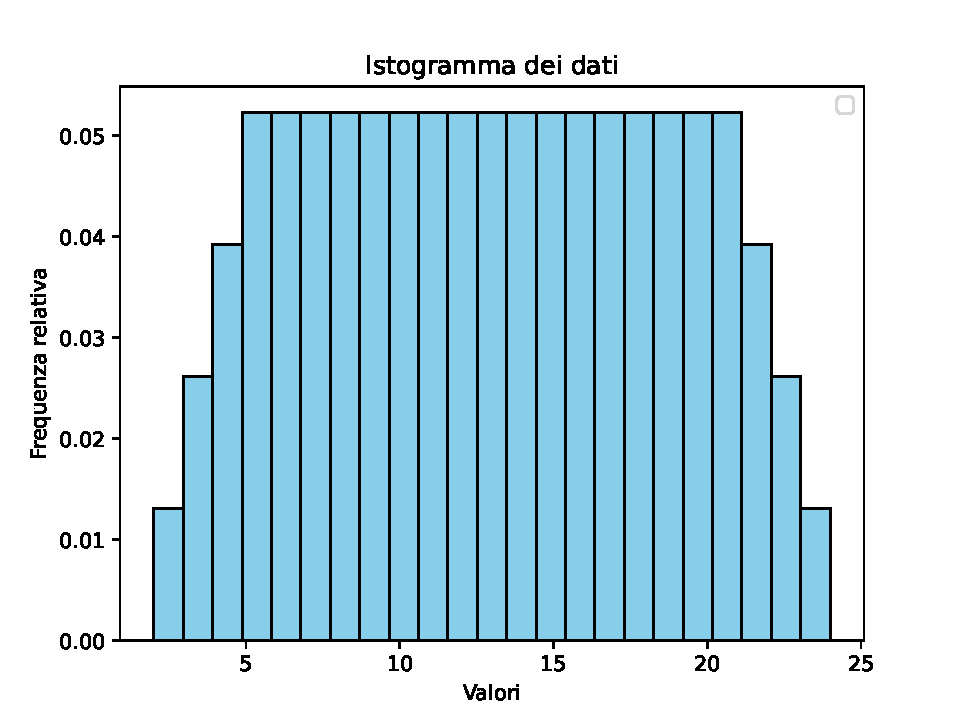
\includegraphics[width=0.75\textwidth]{istogramma1.pdf}
	\caption{L'istogramma normalizzato in figura rappresenta la distribuzione di probabilità della variabile aleatoria $X$. \\
	Valore atteso: $\mu=13$ \\
	Varianza: $\sigma^2=34.5$ \\
	Deviazione Standard: $\sigma=5.87$}
\end{figure}

\subsection{Considerazioni Aggiuntive}
Avendo a disposizione i valori di media $\mu$ e variazione standard $\sigma$ possiamo calcolare le probabilità che la variabile $X$ assuma valori nei seguenti intervalli:
\begin{equation*}
	[\mu-k\sigma, \mu+k\sigma]\ con\ k=1,2,3
\end{equation*} 

Otteniamo così i seguenti risultati:
\begin{itemize}
    \item $k=1: P(X \in [\mu-\sigma, \mu+\sigma]) = 0.55$
    \item $k=2: P(X \in [\mu-2\sigma, \mu+2\sigma]) = 1$
    \item $k=3: P(X \in [\mu-3\sigma, \mu+3\sigma]) = 1$
\end{itemize}





